\section{条件付き模倣学習}
Felipe ら\cite{codevilla2018endtoend}は視覚を入力としたend-to-end学習によって自動運転を行う手法において,右折や左折といった行動ごとにネットワークを変更することで,性能が向上することを報告している.
具体的には2つのネットワークを提案している.
1つ目の\figref{fig:felipe_branched}に示す (a) のネットワークは画像を処理する CNN ,そして CNN の出力と観測,目標方向などのコマンドを入力とする全結合層で構成されている.
2つ目の\figref{fig:felipe_branched}に示す (b) のネットワークは画像を処理する CNN ,そして CNN の出力と観測を目標方向などのコマンドによって全結合層を分ける構造となっている.
シミュレータと実環境両方で実験が行われており,どちらも (b) のネットワークがより優れた結果となった.

\begin{figure}[htbp]
  \centering
  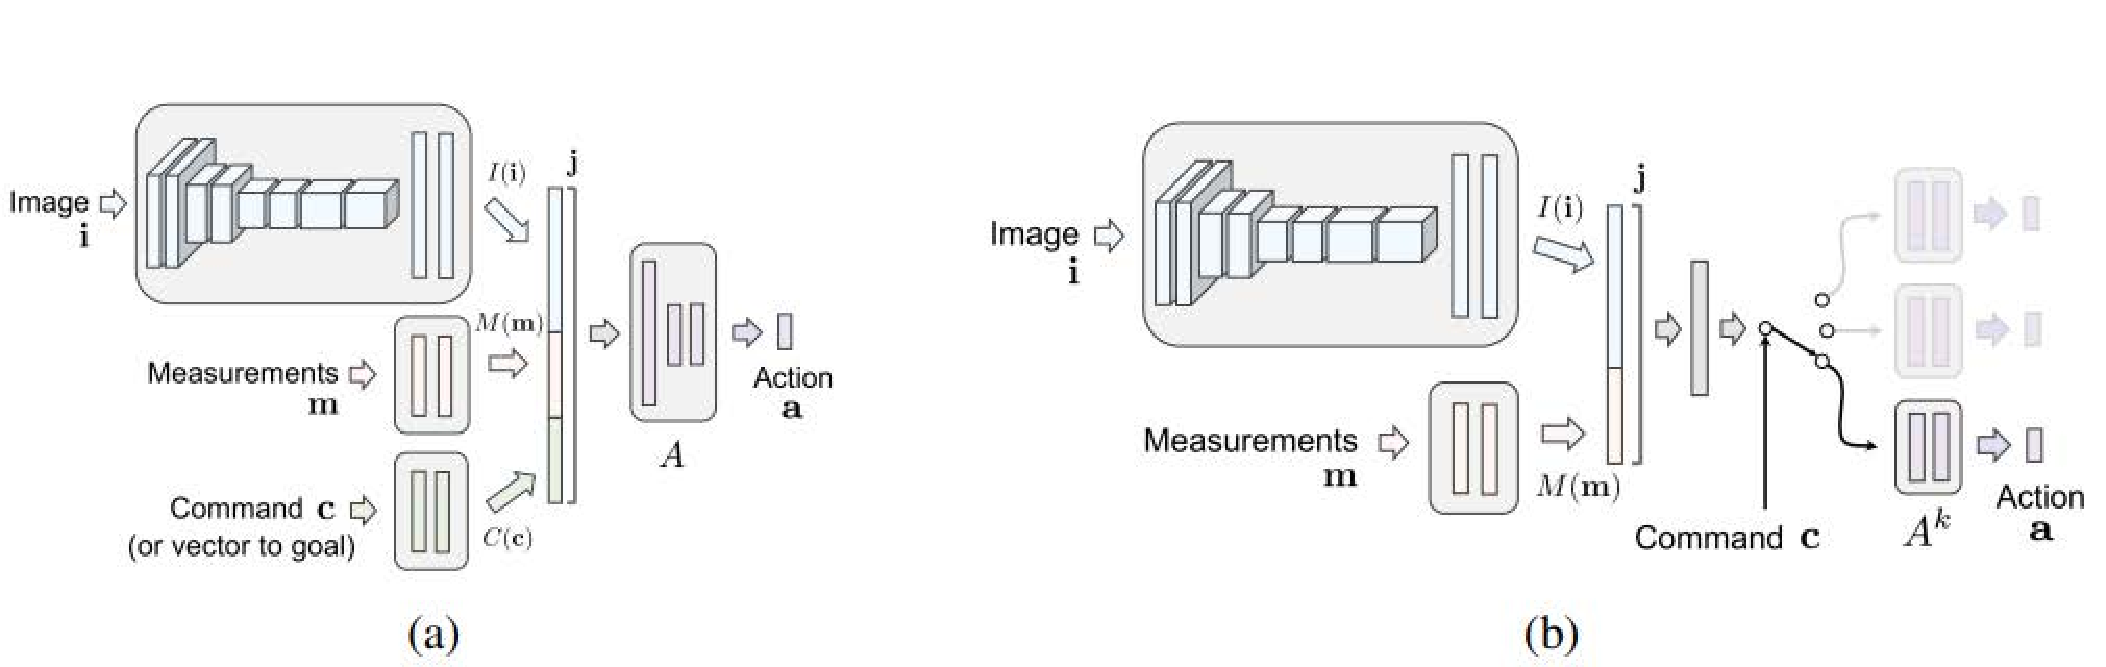
\includegraphics[width=140mm]{images/pdf/other/branched.pdf}
  \caption[Two network architectures for command-conditional imitation learning]{Two network architectures for command-conditional imitation learning 
  \protect\linebreak (Quoted from\cite{codevilla2018endtoend})}
  \label{fig:felipe_branched}
\end{figure}

\clearpage